
\graphicspath{ {\curdir/Graphics/}  }

Quantum computation is a method for performing calculations on data that utilizes additional properties of quantum mechanics that classical computation does not.  Quantum algorithms running on capable systems will be able to perform some calculations in exponentially less time than classical computers will ever be able to.  To realize these speed increases, we need to engineer unprecedented control over thousands of coupled quantum systems.  There are a number of physical systems that have a sufficient degree of isolation from environmental noise that it is possible to consider implementing a quantum computer using them.  These systems include superconducting junctions \cite{Devoret:13}, quantum dots \cite{Kloeffell:13}, trapped neutral atoms \cite{Saffman:10}, and trapped ions.

\section{Motivating Quantum Computing}
In order to quantify the possible speed increase that quantum computers represent, it is useful to refer to the idea of complexity classes in computer science.  Complexity classes are groups of problems that share a similar dependence between the input size of a problem and the time and memory required to solve it using a given computational system.  In Figure~\ref{fig:bqp}, PSPACE, or ``polynomial space'', is the class of problems that can be solved using an amount of memory that is polynomial in the size of the problem on a classical computer.  The size of the problem in this context refers to the size required to represent the inputs of the problem in computer memory.  For example, if the input is a single number, $N$, it can be represented in memory space proportional to $\log{N}$.  For problems that require a large series of numbers as input, the logarithm of each number is approximately the same size and the problem size is often written as the number of input numbers ignoring the approximately constant multiplicative factor.  The ``nondeterministic polynomial'', or NP, complexity class in Figure~\ref{fig:bqp} is the class of problems that can be solved in an amount of computational time that is a polynomial function of the size of the input on a nondeterministic computer.  A nondeterministic computer can take multiple computational paths at every branching point in a program and determine at the end of the computation which path led to a solution.  This class of problems also has the characteristic that a possible solution can be verified in polynomial time on a classical computer.  One of the most important open questions in computer science is whether these problems that can be verified in polynomial time can also be solved in polynomial time on a classical computer, and therefore are also a member of the complexity class P, ``polynomial''.  It is generally believed that these complexity classes are not equal, that is $P \ne NP$, and therefore classical algorithms to efficiently solve NP problems will never be found.  Instead we will have to use algorithms that scale poorly with the size of the problem, and can become difficult to solve even for small scale problems.

\begin{figure}
	\centering
	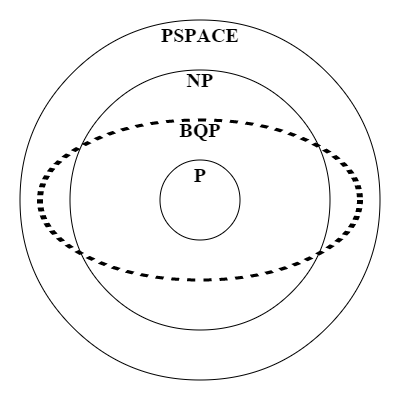
\includegraphics[width=0.4\linewidth] {BQP_complexity_class_diagram}
	\caption[Relationship of BQP complexity class to P, NP, and PSPACE]{The currently believed relationship between the BQP complexity class and other classical computing complexity classes.  BQP includes some problems from NP, as well as some problems from PSPACE outside of NP.  See text for a description of these complexity classes.}
	\label{fig:bqp}
\end{figure}

Quantum algorithms are analyzed as probabilistic algorithms that take into account the probability of the algorithm producing the wrong solution.  The computational class of problems that are easily solved using a quantum computer is named ``bounded error quantum polynomial time'', or BQP.  It is the class of problems solvable in polynomial time on a quantum computer with a probability of failure that is less than $\frac{1}{3}$.  We can see from Figure~\ref{fig:bqp} that quantum computers should be able to efficiently solve some problems that will probably never be efficiently solved classically, including some problems in NP and some problems in PSPACE that are outside of NP.

The most famous quantum algorithm is known as Shor's algorithm.  It is an algorithm for solving the discrete logarithm problem.  The inputs to the problem are two elements, $a$ and $b$, of some finite group, $G$, and the desired output is an exponent, $n$, such that $a^n = b$.  The trivial algorithm is to continuously exponentiate $a$ to higher and higher powers, which takes time proportional to the number of elements of $G$.  Since the input to the problem is two elements of G, the input size of the problem is proportional to $\log \left| G \right|$ and the na\"{\i}ve algorithm takes time proportional to $\left| G \right|$ and exponential in the input size.  Shor's algorithm provides a solution to the discrete logarithm problem that requires only time linear in the size of the input.  

Practically speaking, this problem has applications in cryptography for which groups with size $2^{256}$ or larger are often chosen. Solving this problem is the difficult task that keeps public key cryptographically secured information safe, and it is generally suspected that for sufficiently large groups it will never be solved on classical hardware.  A functional quantum computer of sufficient size could use Shor's algorithm to break all known public key cryptography techniques using a very small amount of computational time. These encryption techniques fall into two groups, those based on factoring large integers and those based on solving for roots of elliptic curves in finite fields.  Both of these problems are easy to solve in one direction, but classically very costly to solve in the opposite direction unless you know a secret piece of information.  Someone desiring to encrypt something can easily compute the result of these calculations for some given parameters, but unless you know the information used to calculate those parameters decrypting the result of the calculation is very difficult.  Both of these known public-key cryptography problems are extremely susceptible to quantum computing, because the secret information can be quickly determined from the calculation parameters.

There are also many other interested quantum algorithms.  Grover's algorithm allows a computer to find a desired item in an unordered list of $N$ items in time proportional to $\sqrt{N}$.  There are also algorithms that allow us to determine the characteristics of quantum black box devices very quickly including the Deutsch-Jozsa algorithm and Simon's algorithm.  There is still ongoing research into finding new computer science problems where quantum computers can outperform classical.

From a physicist's point of view, perhaps the larger motivation for building a quantum computer is the ability to simulate complicated quantum systems.  Trapped ion based quantum computers are beginning to approach being able to find results for physical problems that are very difficult for classical computers to solve.  In particular, frustrated magnetic systems can already be simulated using trapped ions \cite{Islam:13}, but these systems are very difficult to solve classically even for only dozens of particles.  Optical lattices of neutral atoms are also already being used to probe condensed matter states such as Mott insulators and antiferromagnetic states \cite{Bakr:09}.  Simulating full Hamiltonians of complicated systems may remain infeasible on classical computers for decades still, while because of their favorable scaling, quantum computers will be trivially able to do so.

\section{The DiVincenzo Criteria}
\label{sec:divincenzo}

Although there are many systems under investigation as potential quantum computing technologies, I am only going to seriously discuss the possibilities of trapped ion quantum computers.  In order to guide our discussion of how trapped ions represent a possible technology for implementing quantum computation, I will follow the venerable DiVincenzo criteria \cite{DiVincenzo:00}.  These five criteria were proposed by David DiVincenzo in 2000, and describe the basic requirements for a feasible quantum computing architecture.  They place limits on both the physical system chosen to represent quantum information and the technologies that isolate and interact with it.

The operational units of a quantum computer are usually referred to as qubits (short for quantum bits).  Qubits have two possible values $\ket{0}$ and $\ket{1}$ just like classical bits have two possible values 0 and 1, but they can also represent any superposition of those two values.  Two energy states in the ion are chosen to represent these two values.   The populations and coherences of these energy levels are manipulated by applying external fields.  Additionally, quantum computers can work with quantum entangled states of qubits, which is a necessary capability for the additional computational power of quantum computers.

\subsubsection{1. A scalable physical system with well characterized qubits}

The first criteria is unfortunately the one that is most difficult to realize with a trapped ion system.  The qubits themselves, represented by long-lived internal energy states of the ions, are certainly well characterized.  However, the physical system required to trap the ions and generate entanglement between them has proven difficult to scale to large numbers of ions.  Current state of the art systems can simultaneously entangle 14 qubits \cite{Monz:11}, which is already technically very challenging and still of limited use computationally.  The focus of the rest of this thesis will be on one proposal for scaling ion trap systems up to useful number of qubits.

\subsubsection{2. The ability to initialize the state of the qubits to a simple fiducial state, such as $\ket{000...}$} 

This ability is easily realized in trapped ions by tuning the polarization or frequency of a group of lasers to drive transitions from all but one accessible long-lived state, a technique called optical pumping.  The exact details depend on the species being trapped, but are usually very straightforward.  A possible procedure for an ion with a J = 1/2 excited and ground state is outlined in Figure~\ref{fig:optical-pumping}.  

Once these transitions are addressed the population will be pumped to the non-addressed long-lived state by decay from the excited states.  From this optically pumped state the qubit can be transferred to whatever state represents $\ket{0}$ in the proposed computation scheme.  In practice, only a few lasers are often necessary to realize this procedure and the desired state can be initialized with fidelities easily greater than 99\%.

\begin{figure}
	\centering
	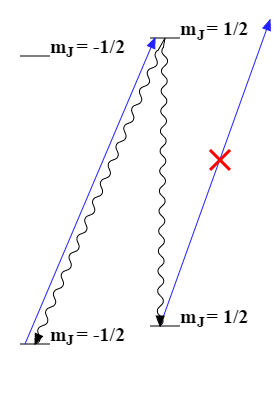
\includegraphics[width=0.35\textwidth]{optical-pumping}
	\caption[Diagram of optical pumping procedure]{Diagram of polarization optical pumping procedure.  Transitions with $\Delta m_J = 1$ are selected by applying $\sigma^+$ polarized light along the angular momentum quantization axis.  Population is pumped to the $m_J = +1/2$ level of the ground state because there are no allowed transition from that state but population can decay there after a transition from the other $m_J$ state.}
	\label{fig:optical-pumping}
\end{figure}

\subsubsection{3. Long relevant decoherence times, much longer than the gate operation time}

Once again the exact details of the implementation depend on the chosen atomic species and isotope, but there are usually several possible long lived states in a given species that could serve as qubits.  In particular, in species with odd nuclear spin there are first order magnetic field insensitive ground state levels with coherence times easily reaching several seconds \cite{Olmschenk:07,Mount:13}.  There are even energy levels separated by optical transition frequencies that have similar decoherence times.  These time scales compare very favorably with gate operation times between 1~$\mu$s and 10~$\mu$s.

\subsubsection{4. A universal set of quantum gates}

A universal set of gates refers to a set of operations that can be performed on the qubits in order to approximate any unitary operator.  In practice, the necessary set can be relatively small and involve only a few single qubit rotations and an entangling operation between qubits.  These kinds of operations are easily accomplished using external electric and magnetic fields with rf and optical frequencies.  The rotations can be accomplished with near-resonant radiation at the qubit energy. The Coulomb interaction between trapped ions provides a strong coupling between their motional energy states that can be used to perform entangling operations.  Fidelities for these operations can be very high, and gate times can be very short \cite{Mount:13}.

\subsubsection{5. A qubit-specific measurement capability}

Ions that can be trapped usually have a strong, cycling optical transition that can scatter millions of photons per second.  By manipulating the internal state of the ions to allow or disallow such a transition, the ions' state can be read out by merely collecting fluorescence.  The state can be determined by collecting fluorescence for tens of milliseconds and applying a simple threshold to separate background fluorescence from fluorescence from the ion (see Figure~\ref{fig:statedetection}).  Read out times as short as 10.5~$\mu$s with 99\% fidelity have been demonstrated \cite{Noek:13}.  This internal state manipulation is often as simple as transferring the ion to a state outside of the decay channels of the driven transition.

\begin{figure}
	\centering
	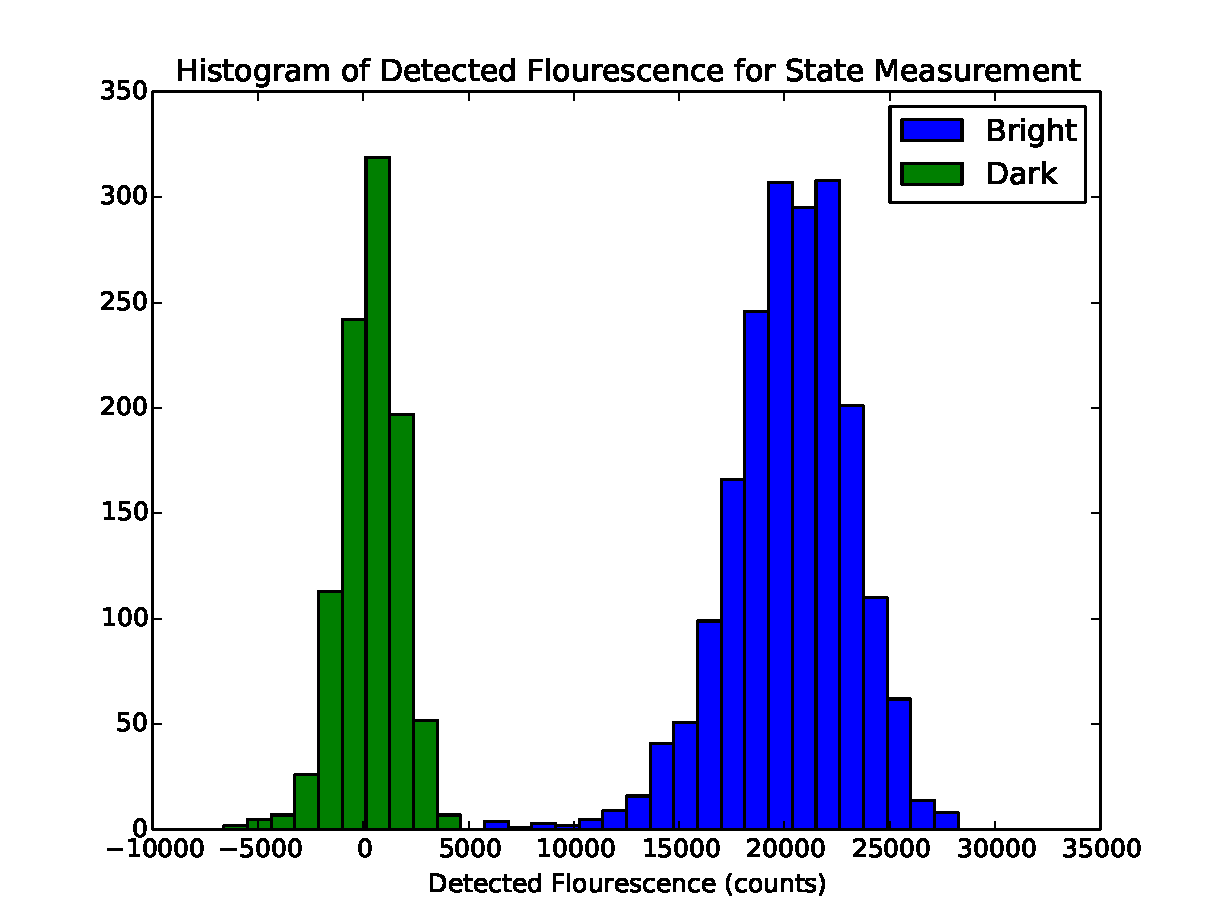
\includegraphics[width=0.6\textwidth]{StateMeasurement}
	\caption[Histogram of collected ion fluoresence for state detection]{Histogram of ion fluorescence detected with an EMCCD in 0.1~s for state detection.  A constant background has been subtracted.  ``Bright'' and ``dark'' states corresponding to the ion being in or out of the cooling cycle can be distinguished with high probability.} 
	\label{fig:statedetection}
\end{figure}

\section{Qubits and Operators}
Initialization and readout of trapped ion quantum systems requires analysis of the atomic structure of the particular choice of species.  Specific lasers and procedures are required for different ions, but only resonant transitions and fluorescence collection are required.  The necessary techniques for our ions will be discussed in Chapter~\ref{sec:ioncool}.  Quantum gates to be performed between out initialization and readout can also be engineered, but we will need to analyze the effects of nonresonant lasers and ion motional modes.  To realize a universal quantum computer we must be able to perform each gate in a universal set of quantum gates.  There are many possible choices for such a set, but I will consider the Hadamard (H), the $\frac{\pi}{8}$ (T), and controlled-not (CNOT) gates.  These gates can be represented as the unitary matrices
\begin{equation}
	U_H = \frac{1}{\sqrt{2}} \left( \begin{array}{cc} 
		1 & 1 \\ 1 & -1 
	\end{array} \right) \quad
	U_T = \left( \begin{array}{cc} 
		1 & 0 \\ 0 & e^{i \frac{\pi}{4}}
	\end{array} \right) \quad
	U_{CNOT} = \left( \begin{array}{cccc}
	1 & 0 & 0 & 0 \\
	0 & 1 & 0 & 0 \\
	0 & 0 & 0 & 1 \\
	0 & 0 & 1 & 0
	\end{array}\right) \mathrm{.}
	\label{eqn:univgates}
\end{equation}
The first two gates are single qubit gates that we must be able to apply to any qubit in the system.  The third is a two qubit entangling gate that we must be able to apply to any pair of qubits in the system.  A mathematical approach to the interaction between light and ions will help clarify how to engineer these gates.  Once we have chosen our two qubit levels, $\ket{0}$ and $\ket{1}$, in a given ion whose energies are $E_0$ and $E_1$, the state of the system can be described by a wavefunction of the form 
\begin{eqnarray}
	\Psi(t) &=& a e^{i \frac{E_0}{\hbar} t} \ket{0} + b e^{i \frac{E_1}{\hbar} t} \ket{1} \\
	&=& \cos( \theta/2 ) \ket{0} + \sin( \theta/2 ) e^{i \phi} e^{i \omega t} \ket{1} \mathrm{,}
\end{eqnarray}
where a and b are arbitrary complex numbers satisfying $\left| a \right|^2 + \left| b \right|^2 = 1$, and $\omega \equiv \frac{E_1 - E_0}{\hbar}$. The second form has dropped an overall phase and reparametrized $a$ and $b$ into angles $\theta$ and $\phi$.  Often such wavefunctions are represented graphically by vectors on the Bloch sphere (see Figure~\ref{fig:bloch}).  The $+\hat{z}$ axis is usually chosen to represent $\ket{1}$, and the $-\hat{z}$ axis to represent $\ket{0}$.  The polar angle of any arbitrary vector is given by $\theta$, while the azimuthal angle is equal to $\phi$.  The Bloch sphere itself is rotating at angular frequency $\omega$.

\begin{figure}
	\centering
	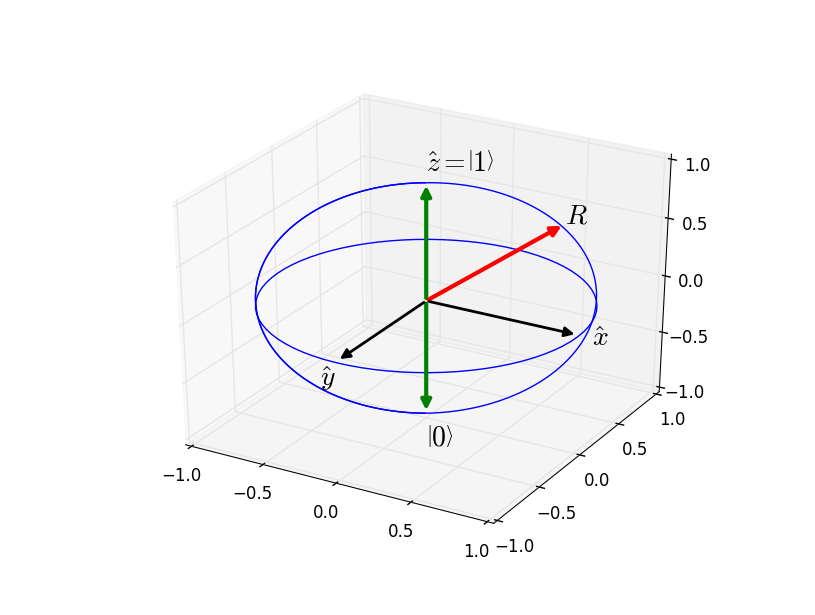
\includegraphics[width=0.7\linewidth]{Bloch_Sphere}
	\caption[Bloch sphere representation of qubit wavefunction]{Vectors on the Bloch sphere can represent any possible qubit state $\Psi = a\ket{0} + b\ket{1}$. The $\hat{z}$ axis represents $\ket{1}$, while the $-\hat{z}$ axis represents $\ket{0}$.  Positions along the equator represent equal population superpositions at different phases $\Psi = \frac{1}{\sqrt{2}}( \ket{0} + e^{i \phi} \ket{1} )$.}
	\label{fig:bloch}
\end{figure}

Rotations are a convenient basis for describing coherent operations on qubits because all decoherence-free operations will preserve $\left| a \right|^2 + \left| b \right|^2 = 1$ and will therefore merely rotate the Bloch representation of each state along the surface of the Bloch sphere.  To perform these rotations using systems with a strong dipole moment, it is only necessary to use an external electric field.  Consider the two level Hamiltonian for our qubit system
\begin{equation}
H = \frac{\hbar}{2} \omega \sigma_z \mathrm{,}
\end{equation}
where $\omega$ is the angular frequency defined above and I have used $\sigma_z$, one of the three Pauli matrices
\[ 
\sigma_x = \left( \begin{array}{cc} 0 & 1 \\ 1 & 0 \end{array} \right) \quad
\sigma_y = \left( \begin{array}{cc} 0 & -i \\ i & 0 \end{array} \right) \quad
\sigma_z = \left( \begin{array}{cc} 1 & 0 \\ 0 & -1 \end{array} \right)\mathrm{.}
\]
We can generally describe coherent interaction of this two level system with an external electric field via the potential
\begin{equation}
	V = \left| \vec{\mu} \cdot \vec{E} \right| \cos{\left( (\omega + \delta) t \right)} \sigma_x \mathrm{,}
\end{equation}
where $\vec{\mu}$ is the ion dipole moment, $\vec{E}$ is the electric field magnitude and polarization, and $\delta$ is the detuning of the electric field oscillation angular frequency from $\omega$.

Consider a qubit system initialized to $\ket{0}$.  Using time dependent perturbation theory, we can find the time derivatives of $a$ and $b$ to be 
\begin{eqnarray}
	\label{eqn:dota}
	\dot{a} &=& -i \Omega b e^{i \delta t} \\
	\label{eqn:dotb}
	\dot{b} &=& -i \Omega a e^{-i \delta t} \mathrm{,}
\end{eqnarray}
where we have dropped the quickly oscillating complex amplitudes and defined $\Omega \equiv \frac{ \vec{\mu} \cdot \vec{E} }{\hbar}$.  For short interaction times we can approximate the probability amplitudes of the two states as constant and let $a(t) \approx 1$ and $b(t) \ll 1$.  In this approximation, the population transferred to the excited state, $\ket{1}$, 
\begin{equation}
	\left| b \right| ^2 = \Omega^2 \frac{\sin^2{ \delta t / 2 }}{\delta^2} \mathrm{.}
	\label{eqn:shortpulses}
\end{equation}
This equation will be useful for using short pulses to make simple measurements of $\Omega$ in later chapters.

The above approximations hold for small population transfers, but in order to analyze the long term behavior we need to simultaneously consider both the excited and ground state occupations.  In order to make a geometric connection we can start by considering
\begin{eqnarray}
	u &=& 2\Re(a b^* e^{i \delta t}) \\
	v &=& 2\Im(a b^* e^{i \delta t}) \\
	w &=& \left| b \right|^2 - \left| a \right|^2
\end{eqnarray}
where $u$, $v$, and $w$ are the x, y, and z components of the Bloch sphere representation of $\ket{\Psi}$ with an additional rotation of the Bloch sphere at angular frequency $\delta$.  Their time derivatives can then be found using Equations~\ref{eqn:dota} and \ref{eqn:dotb} to be
\begin{eqnarray}
	\dot{u} &=& \delta v \\
	\dot{v} &=& -\delta u + \Omega w \\
	\dot{w} &=& -\Omega v
	\label{eqn:wdot}
\end{eqnarray}
Defining $\vec{P} = u \hat{x} + v \hat{y} + w \hat{z}$ to be the vector representing $\ket{\Psi}$, we can write $\dot{\vec{P}} = \vec{P} \times ( \Omega \hat{x} + \delta \hat{z} )$.  This formulation makes it clear that we can coherently control the state of a single qubit by controlling the frequency and amplitude of near resonant electric fields.  These degrees of freedom choose a vector about which the Bloch sphere representation of the qubit state will precess, and choosing the correct time duration allows us to reach any state we desire. 

If we are only interested in the probability of measuring $\ket{1}$ after beginning in $\ket{0}$, we can derive the results easily from Equation~\ref{eqn:wdot}.  The maximum probability to reach $\ket{1}$ can be found by reflecting the $-\hat{z}$ axis across the vector $\vec{W} = \Omega \hat{x} + \delta \hat{z}$, and the rotation speed is determined by the length of $\vec{W}$.  The transition is driven with probability
\begin{equation}
	\left| b \right|^2 = \frac{\Omega^2}{W^2} \sin^2( W t / 2 )
\end{equation}
where we have defined
\begin{equation}
	W^2 \equiv \Omega^2 + \delta^2 \mathrm{.}
\end{equation}
By applying resonant ($\delta$ = 0) electric fields, we see that we can cause population to fully oscillate between $\ket{0}$ and $\ket{1}$.  This behavior is called Rabi oscillation and $\Omega$ is often referred to as the Rabi frequency.  Simply controlling the exposure time of the fields to the ion allows us to perform an arbitrary rotation around the $\hat{y}$ axis on the Bloch sphere.  Given the strength of these couplings in ions, full population transfers can easily be achieved in 1~$\mu$s to 10~$\mu$s with readily available optical or rf power.  By controlling the detuning of the field or by allowing some phase evolution between the field and qubit, we can perform rotations about $\hat{z}$.  Combining the two we can easily implement the H and T gates, or any other set of single qubit gates that we need.

However, the fundamental speed increases available through quantum computation rely on the ability to generate entanglement between qubits.  Without entanglement a quantum computer will not be able to outperform a classical, probabilistic computer.  Therefore, we must have at least one operation which can generate entanglement between our qubits.  A common choice is the controlled NOT operation, which is described by the unitary matrix given in Equation~\ref{eqn:univgates}.  The corresponding classical action can be described as flipping the state of the controlled qubit if the other qubit is set to $\ket{1}$, and otherwise doing nothing.

While single qubit operations are relatively easily engineered in trapped ion systems, implementing entangling operations is significantly more difficult.  The method used to implement them is dependent on the interaction that can be engineered between the qubits themselves.  In trapped ion systems, $N$ ions that are confined in the same trap share $3N$ quantum harmonic oscillator modes of motion coupled via Coulomb forces.  These harmonic oscillator states are used as intermediate states to allow communication between the qubits.  A number of methods for generating entanglement between ions have been proposed including the Cirac-Zoller gate \cite{Cirac:95}, the M{\o}lmer-S{\o}rensen gate \cite{Sorensen:00}, and the Garc\'{i}a-Ripoll gate \cite{GarciaRipoll:03}.  The Garc\'{i}a-Ripoll gate has the most desirable properties including being completely insensitive to the ions motional energy and having a total gate time that can be much quicker than the time scale of the motion of the ions.  However, the optical setup to efficiently implement it is complicated \cite{Mizrahi:13}, and we will instead use the M{\o}lmer-S{\o}rensen gate for the moment.

\begin{figure}
	\centering
	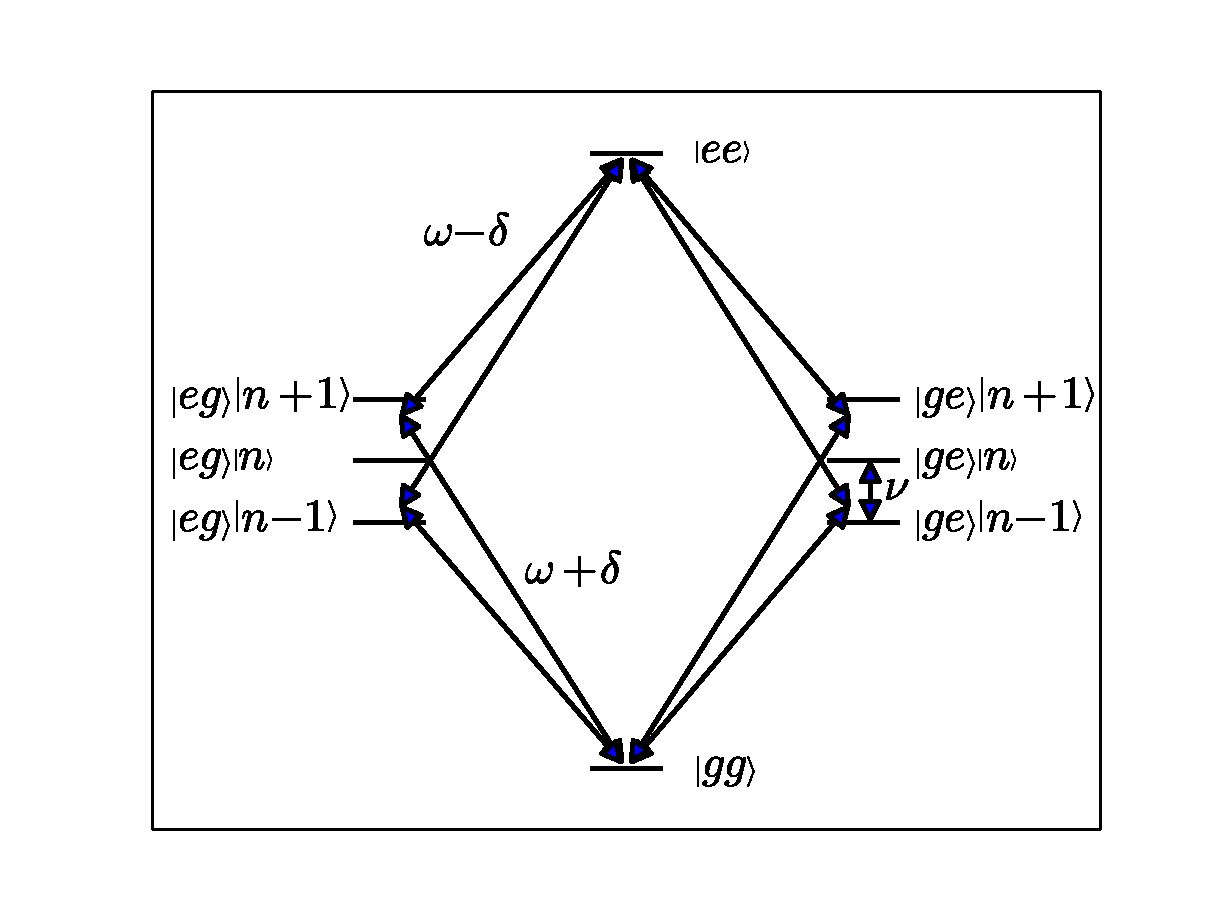
\includegraphics[width=0.7\textwidth]{MolmerSorensen}
	\caption[Diagram of M\o{}lmer-S\o{}rensen gate]{Diagram of relevant energy levels and transitions for implementing the M\o{}lmer-S\o{}rensen gate.  Two optical fields are each applied to two ions at frequencies $\omega \pm \delta$, where $\omega$ is the angular frequency splitting between the qubit levels $\ket{0}$ and $\ket{1}$.  $\delta$ is tuned near but not resonant with the motional mode angular frequency, $\omega_x$.}
	\label{fig:molmersorensen}
\end{figure}

The M{\o}lmer-S{\o}rensen gate is a two qubit entangling gate that uses these motional modes and is tolerant to finite temperature in them.  For a normal mode with angular frequency $\omega_x$ and a qubit angular frequency $\omega$, the two ions are both exposed to two external fields with angular frequencies $\omega \pm \delta$.  When $\delta$ is tuned close to $\omega_x$, these fields excite a virtual phonon into the motional mode and then remove it.  The resulting evolution of the qubit states is independent of the number of motional quanta in the mode, $n$ (for sufficiently small $n$), but the two ions are linked via the exchange of the phonon and must coherently transition together.  The action of this pulse sequence on two qubit states of our qubit levels, $\ket{0}$ and $\ket{1}$, can be described by
\begin{eqnarray}
	\ket{00} &\rightarrow& \cos\left( \frac{\Omega_{MS} t}{2} \right) \ket{00} + i \sin\left( \frac{\Omega_{MS} t}{2} \right) \ket{11} \\
	\ket{11} &\rightarrow& \cos\left( \frac{\Omega_{MS} t}{2} \right) \ket{11} + i \sin\left( \frac{\Omega_{MS} t}{2} \right) \ket{00} \\
	\ket{01} &\rightarrow& \cos\left( \frac{\Omega_{MS} t}{2} \right) \ket{01} - i \sin\left( \frac{\Omega_{MS} t}{2} \right) \ket{10} \\
	\ket{10} &\rightarrow& \cos\left( \frac{\Omega_{MS} t}{2} \right) \ket{10} - i \sin\left( \frac{\Omega_{MS} t}{2} \right) \ket{01} 
\end{eqnarray}
where we have defined
\begin{equation}
	\Omega_{MS} = \frac{(\Omega \eta)^2}{\delta - \omega_x}\mathrm{,}
\end{equation}
and $\Omega$ is the coupling strength of the field to the qubit transition as in Equations~\ref{eqn:dota} and ~\ref{eqn:dotb}, while $\eta = \sqrt{\frac{\hbar}{2 m \omega_x}} k_x$ is the Lamb-Dicke parameter that describes the coupling strength between the photon momentum and each ion's motional states in terms of the ion's mass, $m$, and the photon wavevector in the $\hat{x}$ direction, $k_x$.  Since this transition is independent of the motional energy level of the ion, it can be driven with relatively high temperatures that can easily be reached with simple laser cooling techniques.  The entanglement is even robust against ion heating during the transition and only requires that the ion be cold enough to satisfy $\eta^2 n \ll 1$.  This type of gate has been successfully performed with reasonable fidelities in ion traps \cite{Hayes:12,Hayes:10}.  The M{\o}lmer-S{\o}rensen gate implements an entangling operation, but it is not the easily described CNOT operation from above.  However, by performing single qubit rotations before and after this entangling operation, CNOT gates can be realized.
	
Implementing a quantum algorithm can be thought of as applying a complicated unitary matrix on a number of initialized input and ancillary qubits.  The Solovay-Kitaev algorithm allows us to approximate any such quantum algorithm we want to perform using a sequence of operations drawn from a universal set of quantum gates \cite{Dawson:06}.  This algorithm allows us to construct an approximation with error at most $\epsilon$ to any unitary matrix using a number of simple gates that scales as $\log^2(1 / \epsilon )$.  The approximation can be found efficiently on a classical computer before the algorithm is implemented on a quantum device.  For this reason, we can only concern ourselves with implementing the H, T, and CNOT gates I have described, with the promise that by performing many of these gates we can approximate any algorithm.  The only problem with this course of action is the accumulation of errors by performing millions of these simple gates.  Error rates $<$ 10$^{-4}$ have been demonstrated for single qubit gates in trapped ion systems \cite{Brown:11}, but lower rates will be necessary for more than a few thousand gates.  For complicated quantum algorithms, quantum error correction will be necessary to stop this propagation of error, and maintain the fidelity of the approximation to the algorithm in question.  Quantum error correction was first conceived of by Shor and requires more ancilla qubits for each computational qubit and more simple gates for each operation, but promises a higher total fidelity at the end of the algorithm\cite{Shor:95}.  The techniques have been adapted to many different quantum computing proposals including new, scalable architectures for trapped ions\cite{Oi:06}.

All of the basic requirements for quantum computation have been demonstrated with ion trapping systems using available technology.  The difficulty remains in scaling the number of communicating trapped ions to a sufficiently large number to outperform classical computers.  The number of required ions is not the billions it would take to compete with the number of bits in a classical computer, but instead only a few hundred to a few thousand because of the incredibly efficient quantum algorithms that are available for some difficult problems.  In Chapter~\ref{sec:musiqc}, I will discuss our strategies for reaching these numbers of communicating ions.

